\documentclass[12pt]{article}

\topmargin -40pt
\marginparwidth 0pt
\oddsidemargin  -40pt
\evensidemargin 0pt
\marginparsep 0pt
\textwidth 7.2 in
\textheight  10 in
\hoffset  0.1in

\usepackage{amsthm,amsmath,amssymb,amscd,verbatim,epsfig}
\usepackage{mathptmx}
\usepackage{amsfonts}
%\usepackage{setapace}
\usepackage{graphicx}
\usepackage{bm}
%\usepackage{CJK}
\usepackage{ulem}
\usepackage{multicol}
\usepackage{enumerate}
\usepackage{float}
\usepackage{fontspec}
\usepackage{xeCJK}
\usepackage{graphicx}

\setmainfont{Times New Roman}
\setCJKmainfont{TaipeiSansTCBeta-Regular}
\XeTeXlinebreaklocale "zh"
\XeTeXlinebreakskip = 0pt plus 1pt

\title{Homework 2 of Computational Mathematics}
\author{AM15 黃琦翔 111652028}

\begin{document}
\maketitle
\begin{enumerate}
    \item $x^3 = x + 1\implies x^2 = 1 + \dfrac{1}{x}\implies x = \sqrt{1 + \dfrac{1}{x}} = g(x)$.
    $p_1 = g(p_0) = \sqrt{1 + 1} = \sqrt{2} \approx 1.414$.
    $p_2 = g(p_1) = \sqrt{1 + \dfrac{1}{\sqrt{2}}} \approx 1.3065$.
    $p_3 = g(p_2) \approx 1.3172$.
    $p_4 = g(p_3) \approx 1.326$.
    $p_5 = g(p_4) \approx 1.324$ 
    Then, $p_4$ is the answer that we want to find.

    \item Let $f(x) = x^3 + x - 4$, $f'(x) = 3x^2 + 1 < 49$ for all $x\in [1, 4]$.
    Thus, for $|x - y| < \dfrac{10^{-3}}{49} \approx 2.0409e-5$, $|f(x) - f(y)| < 10^3$.
    Find $n$ s.t. $3 \cdot 2^{-n} < 2.0409e-5$, $n > -\log_2(\dfrac{2.0409e-5}{3}) \approx 17.1653$.
    Thus, the bound of the number of iteration is $18$.
    Then, by python code below, the root is about $1.3787$.

    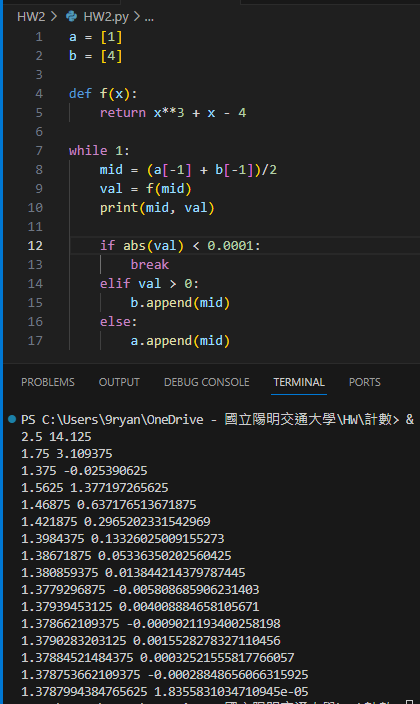
\includegraphics[scale = 0.6]{2024-03-22-214359}

    \item In this question, we let $p_{n+1} = g(p_n)$ and $p = \sqrt[3]{21}$.
    And using the fact that $\dfrac{|p_{n+1}-p|}{|p_n-p|} \approx \dfrac{\lambda |p_n-p|^\alpha}{\lambda |p_{n-1}-p|^\alpha} \approx \left|\dfrac{p_n - p}{p_{n-1}-p}\right|^\alpha$,
    then $\alpha \approx \dfrac{\ln |(p_{n+1} - p)/(p_n - p)|}{\ln |(p_n-p)/(p_{n-1}-p)|}$
    
    \begin{enumerate}
        \item Suppose $p_n\to p$ linearly. 
        $\displaystyle\lim_{n\to\infty} \dfrac{|p_{n+1} - p|}{|p_n - p|} = \displaystyle\lim_{n\to\infty} g'(p_n) = \displaystyle\lim_{n\to\infty} (\dfrac{20p_n^3 + 21}{21p_n^2})' = \dfrac{20}{21} - \dfrac{2}{p^3} = \dfrac{20}{21} - \dfrac{2}{21} = \dfrac{6}{7}$ is constant.
        Thus, it truely converges linearly.

        \item $\displaystyle\lim_{n\to\infty} g'(p_n) = 1 - \dfrac{1}{3} - \dfrac{14}{p^3} = \dfrac{2}{3} - \dfrac{2}{3} = 0$.
        Thus, it converges sublinearly.

        \item $\displaystyle\lim_{n\to\infty} g'(p_n) = 1 - \dfrac{2p^5 - 84p^3 + 21p^2 + 441}{(p^2-21)^2}$

        \item $\displaystyle\lim_{n\to\infty} |g'(p_n)| = |\dfrac{-21\cdot \frac{1}{2}}{p^{3/2}}| = \dfrac{1}{2}$.
        Then, $\displaystyle\lim_{n\to\infty} \dfrac{|g''(p)|}{2} = $
    \end{enumerate}
\end{enumerate}
\end{document}
